\documentclass[problems]{esg8012pset} 
  \usepackage{amsmath}
  \usepackage{amssymb}
  \usepackage{enumerate}
  \usepackage{graphicx}
  \usepackage{hyperref}
  %\usepackage{siunitx}
  \providecommand{\uvec}[1]{{\hat{\bf{#1}}}}
  \usepackage{pgf,tikz}
  \usetikzlibrary{arrows}
  \usepackage{wasysym}
  \makeatletter
  \newcommand{\interitemtext}[1]{%
    \begin{list}{}
     {\itemindent=0mm\labelsep=0mm
     \labelwidth=0mm\leftmargin=0mm
     \addtolength{\leftmargin}{-\@totalleftmargin}}
      \item #1
    \end{list}
  }
  \makeatother
  \renewcommand{\d}{\,d}
  \providecommand{\norm}[1]{\lVert#1\rVert}
\classname{Physics 8.012} 
\semester{Fall 2010} 
\problemsetnumber{11} 
\date{\today } 
\duedate{Friday, December 3} 
\readingassignment{Kleppner and Kolenkow, \emph {An Introduction to Mechanics}, Chapters Seven and Eight} 
\begin{document}
\section{Problem \thesection: K\&K 7.1}
  A thin hoop of mass $m$ and radius $R$ rolls without slipping about the $z$ axis. It is supported by an axle of length $R$ through its center. The hoop circles around the $z$ axis with angular speed $\Omega$. (Note: the moment of inertia of a hoop for an axis along its diameter is $(1 / 2)mR^2$.)
  \begin{center}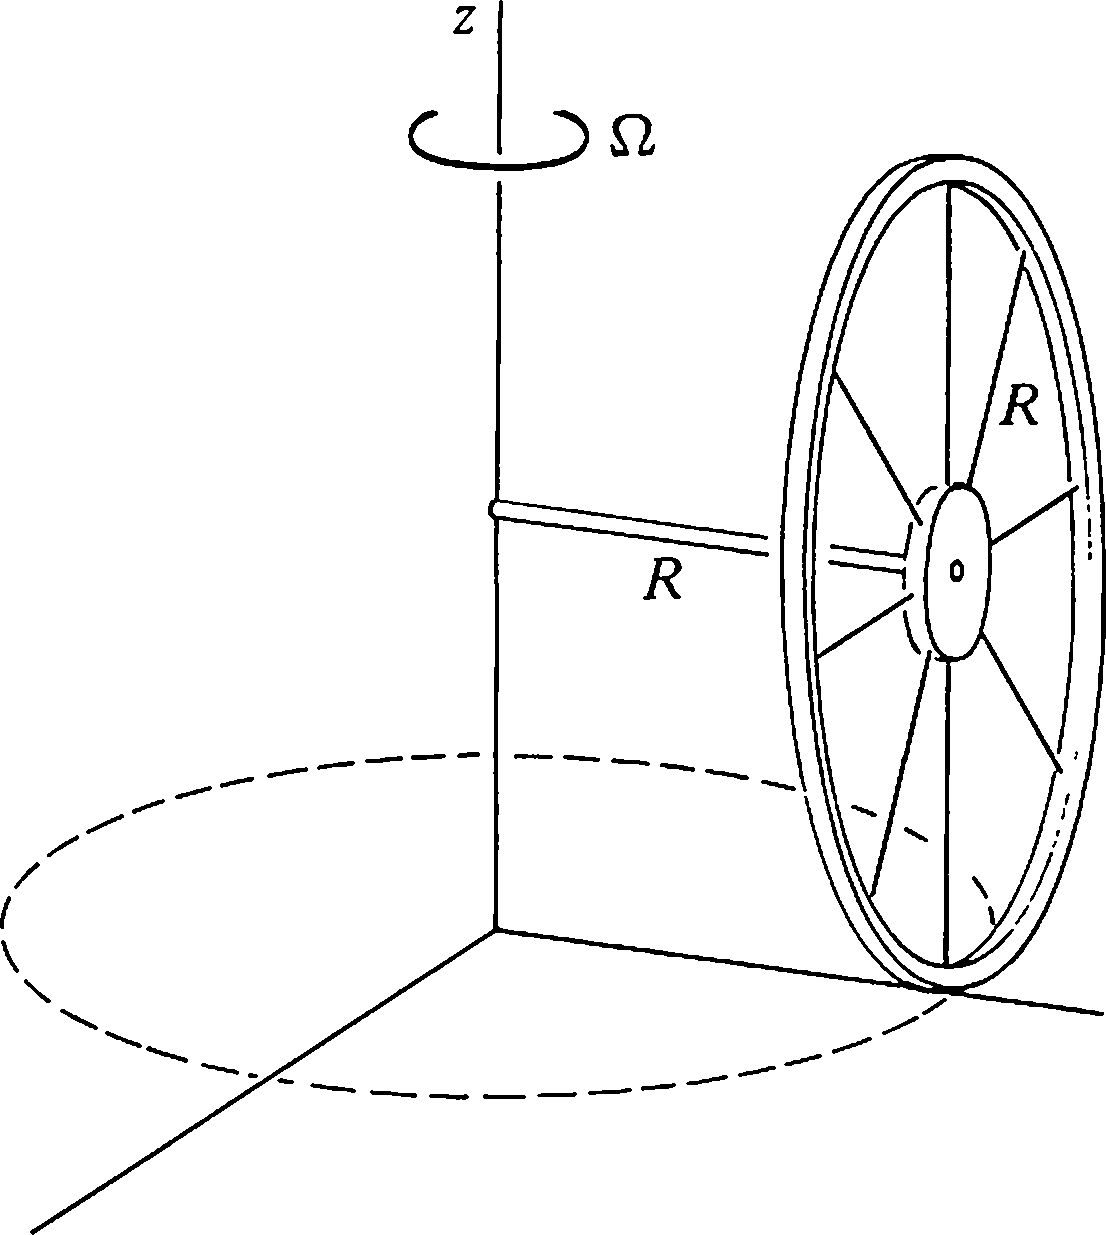
\includegraphics[width=0.4\textwidth]{ps11_1}\end{center}
  \begin{enumerate}[(a)]
    \item What is the instantaneous angular velocity $\vec \omega$ of the hoop? Specify the direction and magnitude.
    \item What is the angular momentum $\vec L$ of the hoop about a point where the axle meets the $z$ axis? Is $\vec L$ parallel to $\vec \omega$?
  \end{enumerate}
\section{Problem \thesection: K\&K 7.3}
  A gyroscope wheel is at one end of an axle of length $l$. The other end of the axle is suspended from a string of length $L$. The wheel is set into motion so that it executes uniform precession in the horizontal plane. The wheel has mass $m$ and moment of inertia about its center of mass $I_\text{cm}$. Its spin angular velocity is $\omega_s$. Neglect the mass of the shaft and the mass of the string. Find the angle $\beta$ that the string makes with the vertical. Assume that $\beta$ is so small that approximations like $\sin\beta \cong \beta$ are justified.
  \begin{center}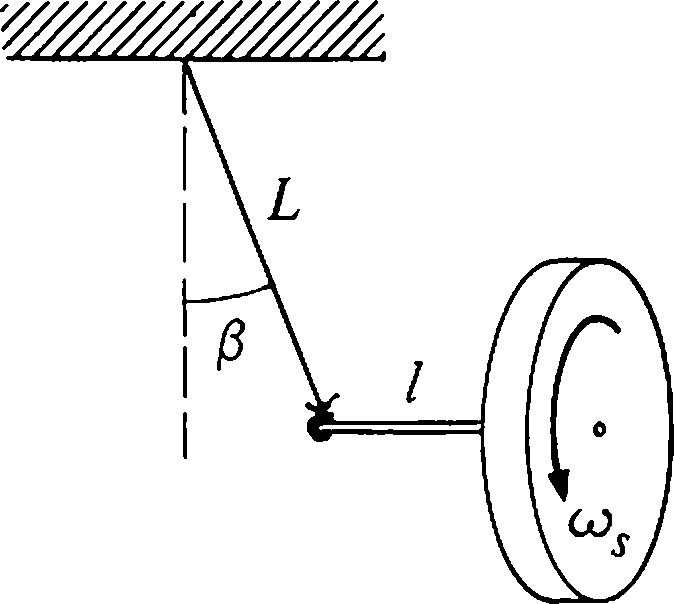
\includegraphics[width=0.2\textwidth]{ps11_2}\end{center}
\section{Problem \thesection: K\&K 7.5}
  When an automobile rounds a curve at high speed, the loading (weight distribution) on the wheels is markedly changed. For sufficiently high speeds the loading on the inside wheel goes to zero, at which point the car starts to roll over. The tendency can be avoided by mounting a large spinning flywheel on the car.
  \begin{enumerate}[(a)]
    \item In what direction should the flywheel be mounted, and what should be the sense of rotation, to help equalize the loading? (Be sure that your method works for cars turning in either direction.)
    \item Show that for a disk-shaped flywheel of mass $m_w$ and radius $R$, the requirement for equal loading is that the angular velocity of the flywheel, $\omega_s$, is related to the velocity of the car $v$ by $$\omega_s = 2v\frac{m_T L}{m_w r^2}$$ where $m_T$ is the total mass of the car and flywheel, and $L$ is the height of the center of mass of the car (including the flywheel) above the road. Assume the road is unbanked.
  \end{enumerate}
\section{Problem \thesection: K\&K 7.8}
  A child's hoop of mass $m$ and radius $b$ rolls in a straight line with velocity $v$. Its top is given a light tap with a stick at right angles to the direction of motion. The impulse of the blow is $I$.
  \begin{enumerate}[(a)]
    \item Show that this results in a deflection of the line of rolling by an angle $\phi = I / m v$, assuming that the gyroscopic approximation holds and neglecting friction with the ground.
    \item Show that the gyroscopic approximation is valid provided $F \ll mv^2 / b$, where $F$ is the peak applied force.
  \end{enumerate}
\section{Problem \thesection: K\&K 8.1}
  A uniform thin rod of length $L$ and mass $m$ is pivoted at one end. The pivot is attached to the top of a car accelerating at rate $A$.
  \begin{center}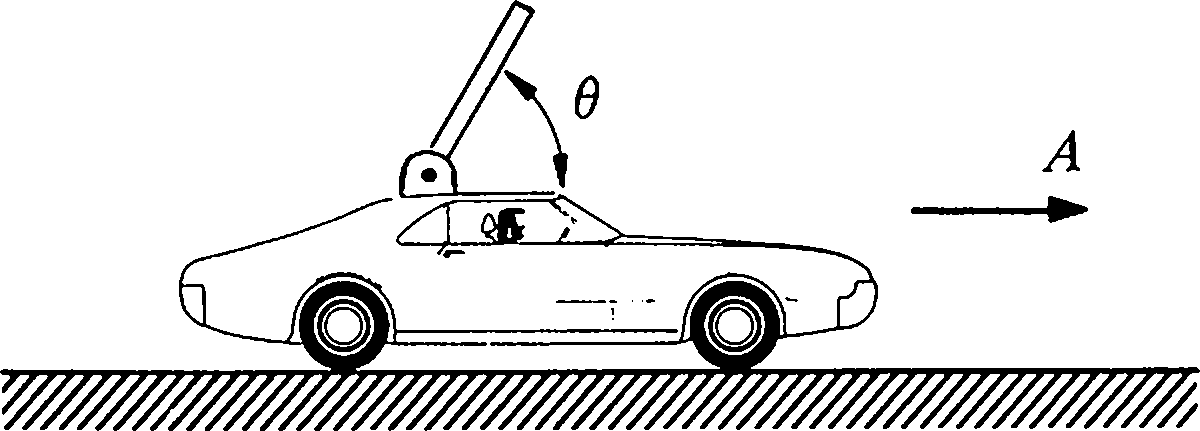
\includegraphics[width=0.5\textwidth]{ps11_3}\end{center}
  \begin{enumerate}[(a)]
    \item What is the equilibrium value of the angle $\theta$ between the rod and the top of the car?
    \item Suppose that the rod is displaced a small angle $\phi$ from equilibrium. What is its motion for small $\phi$?
  \end{enumerate}
\section{Problem \thesection: }
  A particle of mass $m$ slides without friction on the inside of a cone. The axis of the cone is vertical and gravity points downward. The apex half-angle of the cone is $\beta$. The cone is rotating about the vertical axis with angular velocity $\vec \Omega = \Omega \hat k$.  The particle travels in a circular orbit with radius $r$ in the horizontal plane with a constant but unknown speed $(v_\theta)_\text{rot} = r\omega_\text{rot}$ as measured in the rotating reference frame.
  \begin{enumerate}[(a)]
    \item What is the direction of the Coriolis force $\vec F_{cor} = -2 m \vec \Omega \times \vec v_\text{rot}$?
    \item What is the direction of the centrifugal force $\vec F_{cent} = -m \vec \Omega \times (\vec \Omega \times \vec r)$?
    \item What is the angular velocity $\omega_\text{rot}$ of the particle in the rotating reference frame?
  \end{enumerate}
\section{Problem \thesection: K\&K 8.10}
  The acceleration due to gravity measured in an earthbound coordinate system is denoted by $g_0$. However, because of the earth's rotation, $g$ from the true acceleration due to gravity $g_0$. Assuming that the earth is perfectly round, with radius $R_e$ and angular velocity $\Omega_e$, find $g$ as a function of latitude $\lambda$. (Assuming the earth to be round is actually not justified; the contributions to the variation of $g$ due to the polar flattening is comparable to the effect calculated here.)
\section{Problem \thesection: K\&K 8.12}
  A pendulum is rigidly fixed to an axle held by two supports so that it can only swing in a plane perpendicular to the axle. The pendulum consists of a mass $m$ attached to a massless rod of length $l$. The supports are mounted on a platform which rotates with constant angular velocity $\Omega$. Find the pendulum's frequency assuming the amplitude is small.
  \begin{center}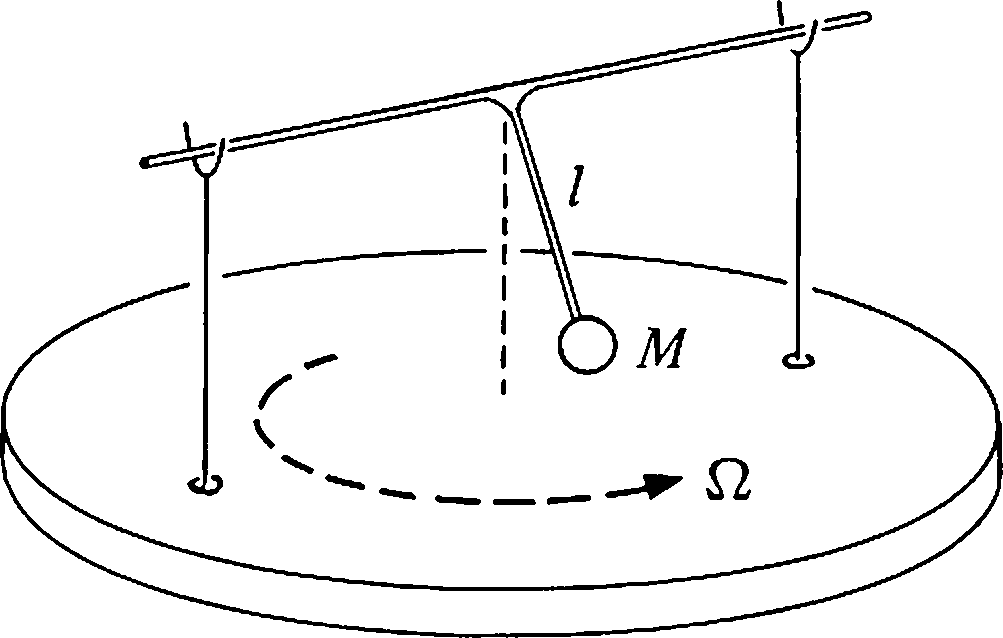
\includegraphics[width=0.4\textwidth]{ps11_4}\end{center}
\end{document}
